\documentclass[final]{beamer}
\usepackage[scale=1.4,orientation=landscape,size=a0]{beamerposter}
\usepackage{graphicx}
\usepackage{booktabs}
\usepackage{xcolor}
\usepackage{array}
\usepackage{colortbl}
\usepackage{tikz}

% ---- Colors ----
\definecolor{posterOrange}{RGB}{217,119,6}
\definecolor{lightGray}{RGB}{249,250,251}
\definecolor{borderGray}{RGB}{229,231,235}

% ---- Beamer theme ----
\setbeamertemplate{navigation symbols}{}
\setbeamertemplate{headline}{}
\setbeamertemplate{footline}{}
\setbeamercolor{background canvas}{bg=white}

\setbeamercolor{block title}{fg=white, bg=posterOrange}
\setbeamercolor{block body}{fg=black, bg=lightGray}
\setbeamerfont{block title}{size=\large, series=\bfseries}
\setbeamerfont{block body}{size=\normalsize}

\setbeamertemplate{block begin}{
  \vskip0.5ex
  \begin{beamercolorbox}[rounded=false, shadow=false, leftskip=0.8cm, rightskip=0.8cm, ht=2.8ex, dp=1.2ex]{block title}%
    \usebeamerfont{block title}\insertblocktitle
  \end{beamercolorbox}
  \usebeamerfont{block body}
  \begin{beamercolorbox}[rounded=false, shadow=false, leftskip=0.8cm, rightskip=0.8cm, sep=0.6cm, vmode]{block body}%
}
\setbeamertemplate{block end}{
  \end{beamercolorbox}
  \vskip0.5ex
}

% ---- Orange bullet ----
\newcommand{\obullet}{\textcolor{posterOrange}{\textbullet}}
\newcommand{\oarrow}{\textcolor{posterOrange}{$\rightarrow$}}

\begin{document}
\begin{frame}[t]

% =============================================================================
% HEADER
% =============================================================================
\begin{beamercolorbox}[wd=\paperwidth, leftskip=2.5cm, rightskip=2.5cm, vmode]{white}
  \color{posterOrange}
  \vspace{1.2cm}
  {\fontsize{72}{86}\selectfont\bfseries FoundationStereo: Zero-Shot Stereo Matching}\par
  \vspace{0.3cm}
  \textcolor{black}{\rule{\dimexpr\paperwidth-5cm\relax}{4pt}}\par
  \vspace{0.4cm}
  \color{black}
  {\fontsize{28}{34}\selectfont
    \textbf{Based on:} Bowen Wen, Matthew Trepte, Joseph Aribido, Jan Kautz, Orazio Gallo, Stan Birchfield --- NVIDIA}\par
  \vspace{0.25cm}
  {\fontsize{26}{32}\selectfont
    \textbf{Presented by:} Danil Smirnov, Federico Cognolatto
    \quad\textbullet\quad 3D Data Processing Poster Session
    \quad\textbullet\quad University of Padova, 2026}\par
  \vspace{1cm}
\end{beamercolorbox}

\vspace{0.5cm}

% =============================================================================
% ROW 1
% =============================================================================
\begin{columns}[t, totalwidth=\paperwidth]
  \hspace{1cm}

  % --- Column 1: Motivation + Key Contributions ---
  \begin{column}{0.30\paperwidth}

    \begin{block}{Motivation}
      Many deep stereo matching models still rely on \textbf{per-domain fine-tuning}
      to achieve competitive performance.
      \begin{itemize}\setlength\itemsep{0.4em}
        \item[\obullet] \textbf{Sim-to-real gap:} Synthetic training fails on real scenes
        \item[\obullet] \textbf{Challenging structures:} Reflections, textureless, thin objects
        \item[\obullet] \textbf{Weak zero-shot:} Poor generalization to unseen domains
      \end{itemize}
    \end{block}

    \vspace{0.6cm}

    \begin{block}{Key Contributions}
      \vspace{0.2cm}
      \begin{enumerate}\setlength\itemsep{0.6em}
        \item \textbf{FoundationStereo:} Stereo foundation model with strong zero-shot generalization
        \item \textbf{FSD Dataset:} 1M synthetic stereo pairs with high diversity
        \item \textbf{Side-Tuning Adapter:} Adapts DepthAnythingV2 for stereo matching
        \item \textbf{Attentive Hybrid Cost Filtering:} Local + global reasoning
      \end{enumerate}
      \vspace{0.2cm}
    \end{block}

  \end{column}
  \hspace{0.8cm}

  % --- Column 2: Architecture Overview ---
  \begin{column}{0.30\paperwidth}

    \begin{block}{Architecture Overview}
      \begin{center}
        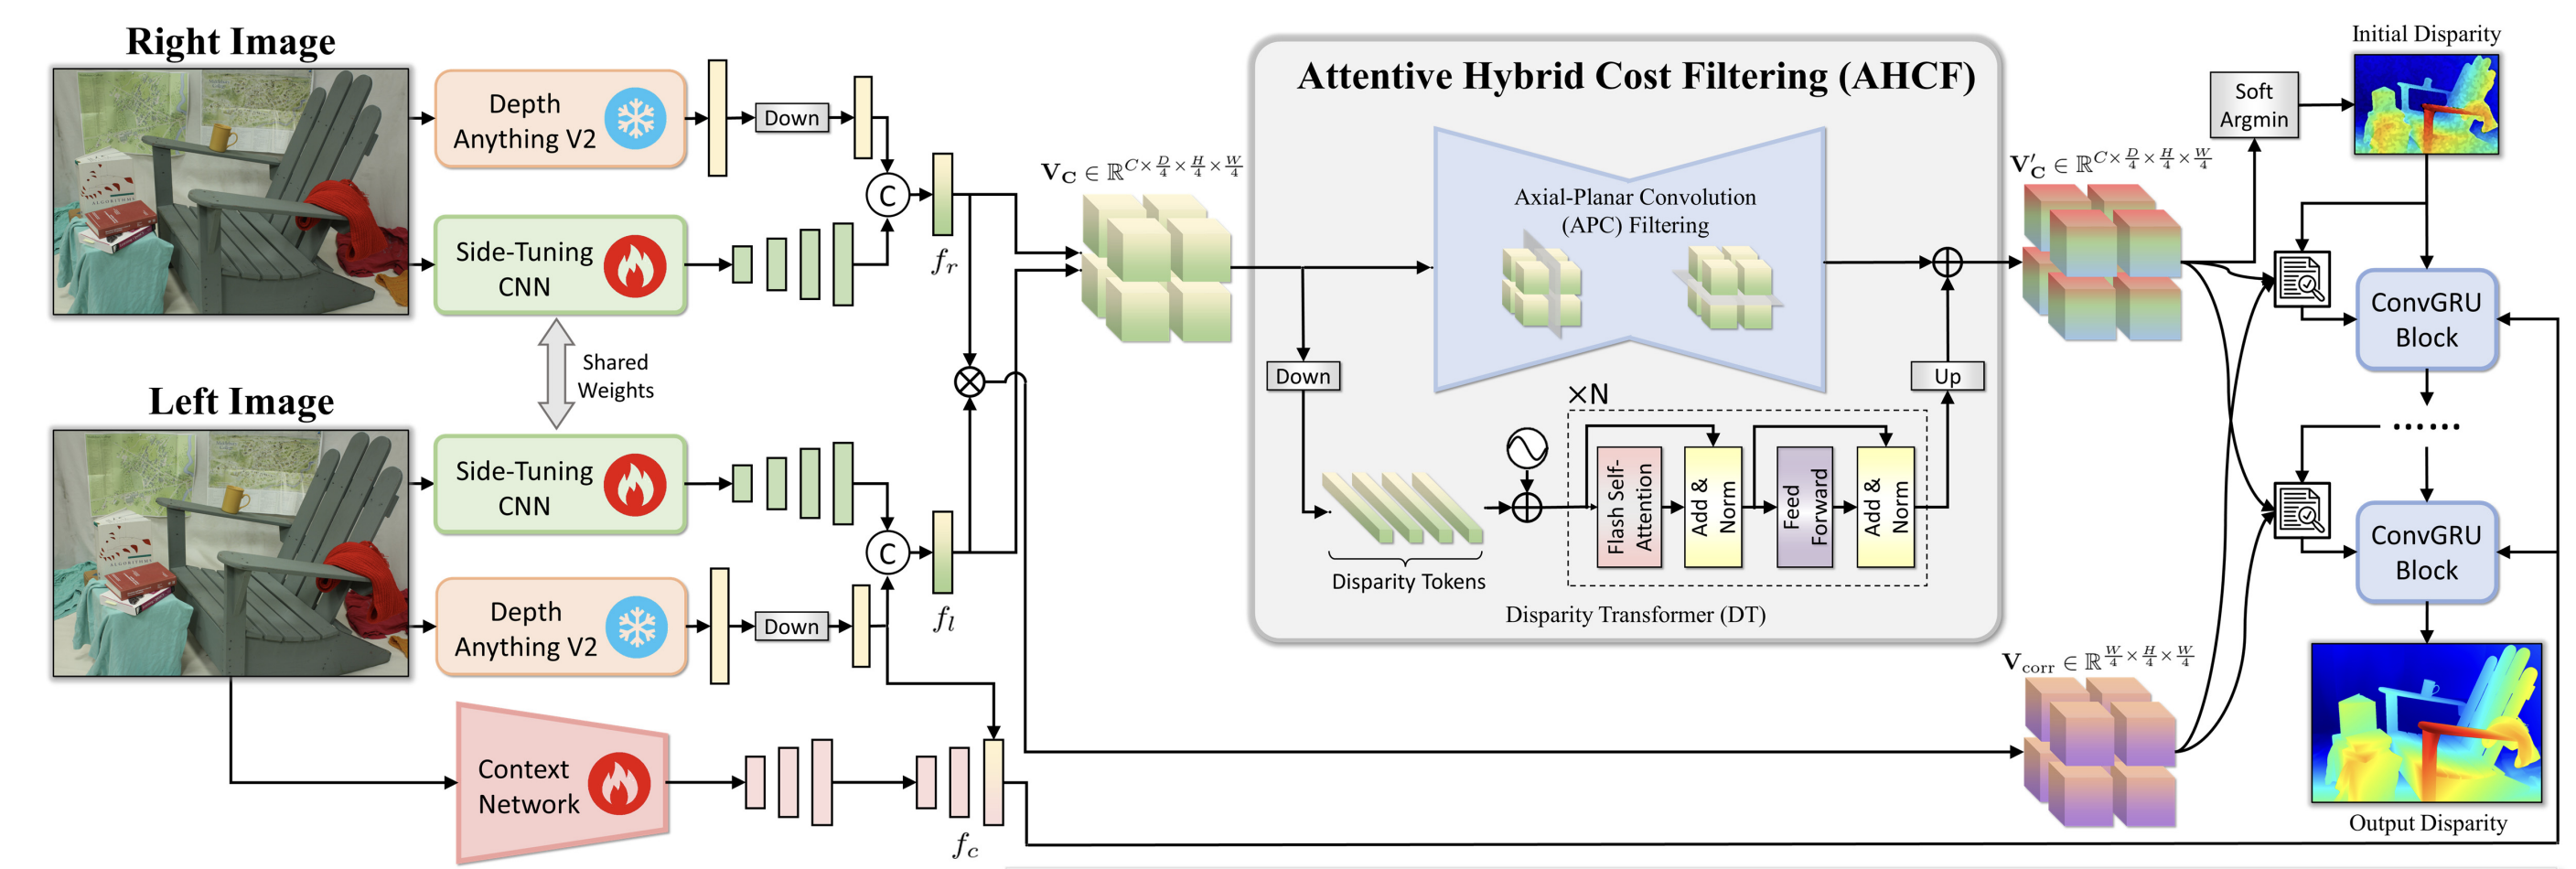
\includegraphics[width=0.95\linewidth]{../src/imports/Figure2.png}
      \end{center}
      \vspace{0.5cm}
      \begin{tabular}{cccc}
        \cellcolor{posterOrange}\color{white}\textbf{Step 1} &
        \cellcolor{posterOrange}\color{white}\textbf{Step 2} &
        \cellcolor{posterOrange}\color{white}\textbf{Step 3} &
        \cellcolor{posterOrange}\color{white}\textbf{Step 4} \\
        \cellcolor{posterOrange}\color{white}Feature Extraction &
        \cellcolor{posterOrange}\color{white}Hybrid Cost Volume &
        \cellcolor{posterOrange}\color{white}Cost Filtering &
        \cellcolor{posterOrange}\color{white}GRU Refinement
      \end{tabular}
      \vspace{0.2cm}
    \end{block}

  \end{column}
  \hspace{0.8cm}

  % --- Column 3: Key Ideas ---
  \begin{column}{0.30\paperwidth}

    \begin{block}{Key Ideas}
      \vspace{0.3cm}
      {\color{posterOrange}\rule{4pt}{1.2em}}\hspace{0.5em}%
      \textbf{Side-Tuning Adapter (STA)}\par
      \vspace{0.2cm}
      \hspace{0.9cm}Adapts monocular depth features from \textbf{DepthAnythingV2}
      for stereo matching through lightweight adapters.

      \vspace{0.6cm}

      {\color{posterOrange}\rule{4pt}{1.2em}}\hspace{0.5em}%
      \textbf{Attentive Hybrid Cost Filtering}\par
      \vspace{0.2cm}
      \begin{itemize}\setlength\itemsep{0.3em}
        \item[\oarrow] \textbf{Axial-Planar Conv:} Efficient spatial + disparity cost-volume filtering
        \item[\oarrow] \textbf{Disparity Transformer:} Long-range reasoning over disparity space
      \end{itemize}

      \vspace{0.5cm}
      \begin{center}
        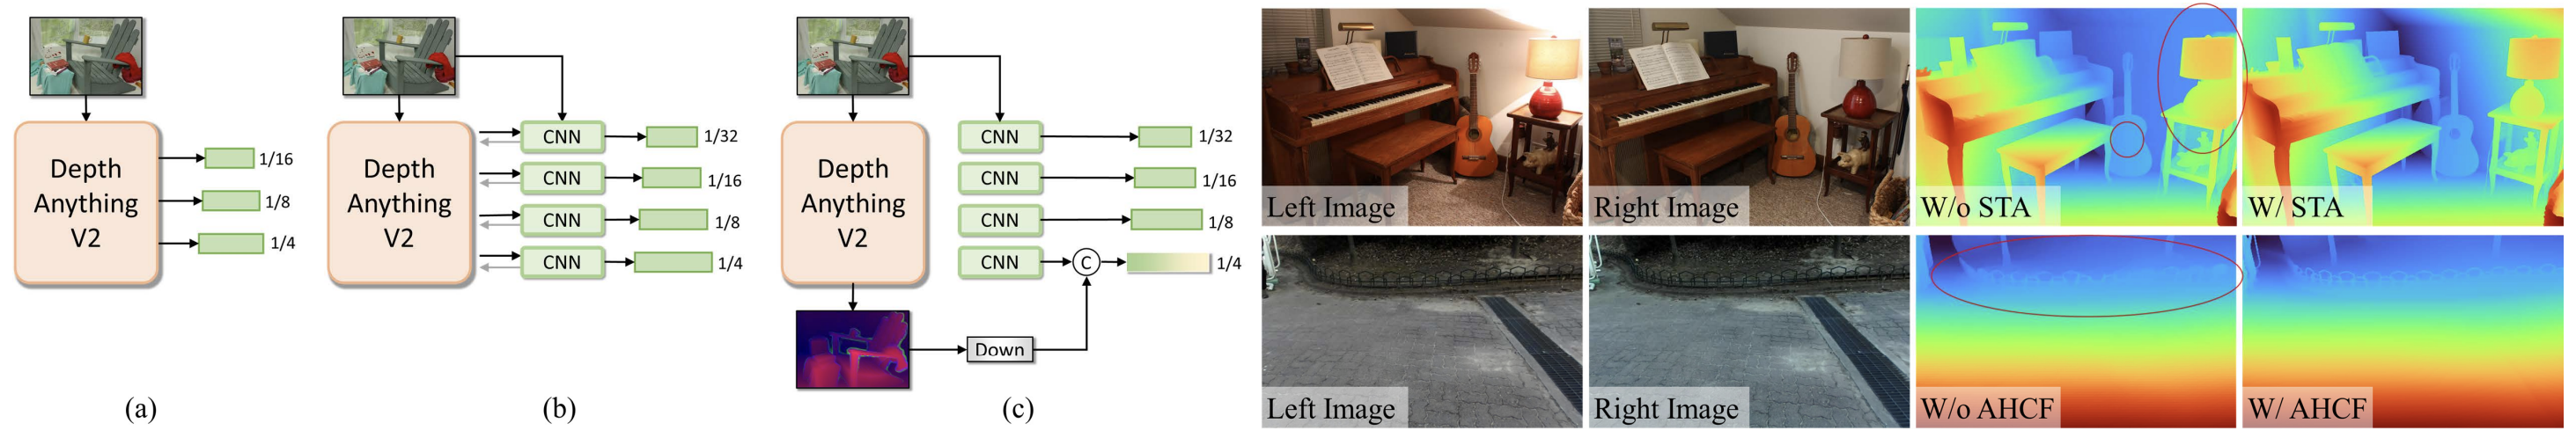
\includegraphics[width=0.9\linewidth]{../src/imports/Figure3.png}
      \end{center}
    \end{block}

  \end{column}
  \hspace{1cm}
\end{columns}

\vspace{0.8cm}

% =============================================================================
% ROW 2
% =============================================================================
\begin{columns}[t, totalwidth=\paperwidth]
  \hspace{1cm}

  % --- Column 1: FSD Dataset ---
  \begin{column}{0.30\paperwidth}

    \begin{block}{FSD Dataset}
      \textbf{1 million stereo pairs} rendered via NVIDIA Omniverse with high realism.

      \vspace{0.5cm}
      \begin{center}
        \begin{tabular}{cc}
          \textcolor{posterOrange}{\fontsize{40}{48}\selectfont\bfseries 1280$\times$720} &
          \textcolor{posterOrange}{\fontsize{40}{48}\selectfont\bfseries 1M} \\
          Resolution & Stereo Pairs
        \end{tabular}
      \end{center}

      \vspace{0.4cm}
      \begin{itemize}\setlength\itemsep{0.2em}
        \item[\obullet] \textbf{Scenes:} Indoor, outdoor, driving, flying
        \item[\obullet] \textbf{Diversity:} Baselines, intrinsics, lighting
        \item[\obullet] \textbf{Self-curation:} Removes ambiguous synthetic stereo pairs
      \end{itemize}

      \vspace{0.4cm}
      \begin{center}
        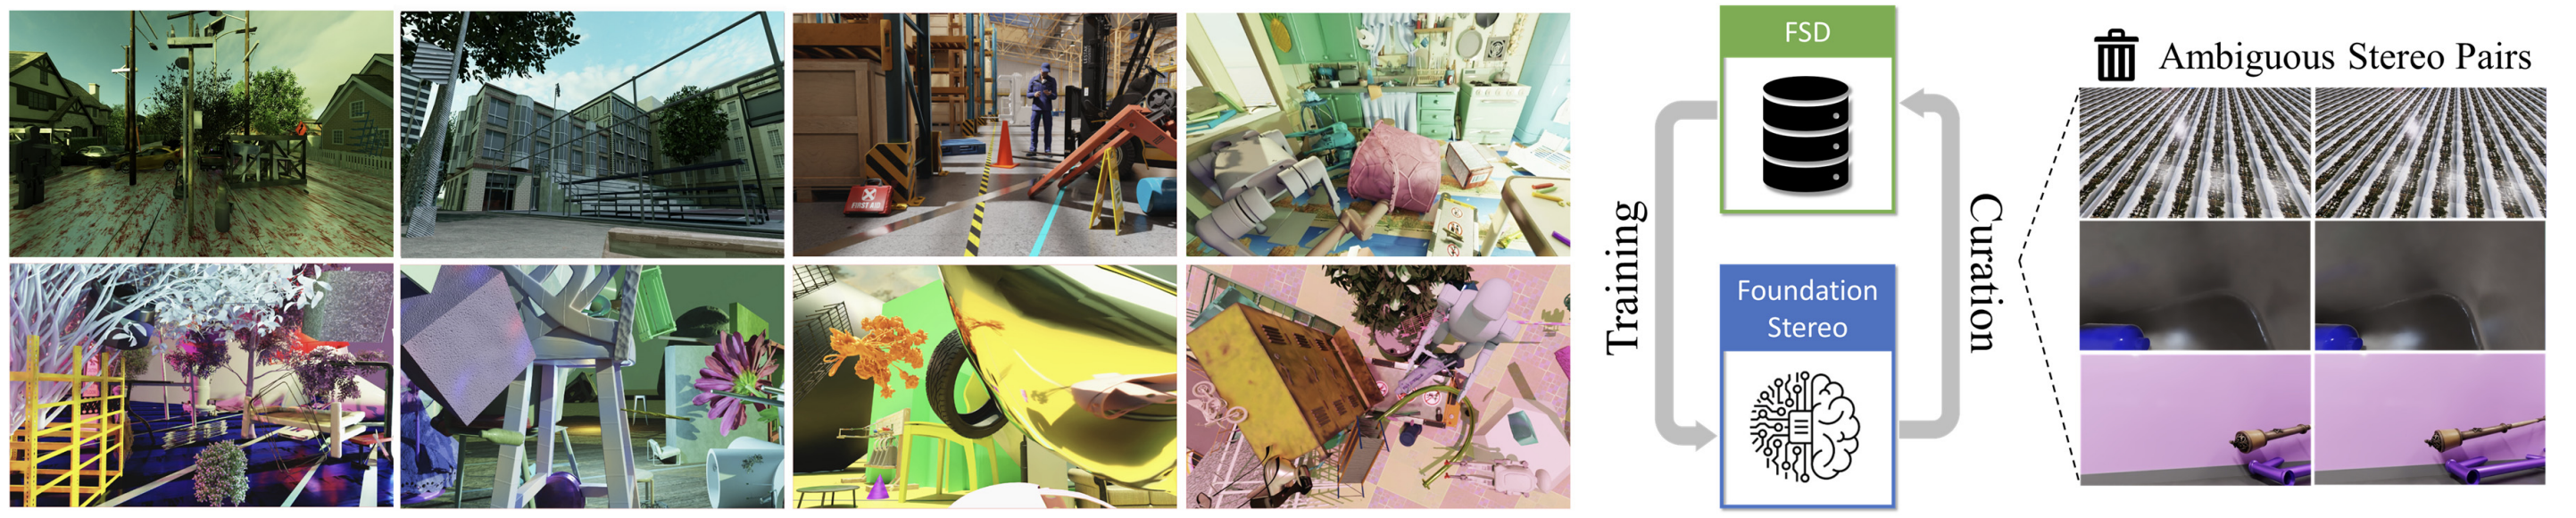
\includegraphics[width=0.9\linewidth]{../src/imports/Figure4.png}
      \end{center}
    \end{block}

  \end{column}
  \hspace{0.8cm}

  % --- Column 2: Zero-Shot Results ---
  \begin{column}{0.30\paperwidth}

    \begin{block}{Zero-Shot Results}
      \textbf{State-of-the-art zero-shot performance} without target-domain fine-tuning.
      \vspace{0.5cm}

      \begin{center}
      \begin{tabular}{lcc}
        \rowcolor{posterOrange}
        \color{white}\textbf{Dataset} &
        \color{white}\textbf{Metric $\downarrow$} &
        \color{white}\textbf{FoundationStereo} \\
        \rowcolor{white}
        Middlebury & BP-2 & \textbf{1.1} \\
        \rowcolor{lightGray}
        ETH3D & BP-1 & \textbf{0.5} \\
        \rowcolor{white}
        KITTI-12 & D1 & \textbf{2.3} \\
        \rowcolor{lightGray}
        KITTI-15 & D1 & \textbf{2.8} \\
      \end{tabular}
      \end{center}

      \vspace{0.6cm}
      \colorbox{posterOrange!15}{%
        \begin{minipage}{0.88\linewidth}
          \vspace{0.3cm}
          \hspace{0.3cm}{\small Lower is better. Values are error rates (\%).}
          \vspace{0.3cm}
        \end{minipage}
      }
    \end{block}

  \end{column}
  \hspace{0.8cm}

  % --- Column 3: In-the-Wild Results ---
  \begin{column}{0.30\paperwidth}

    \begin{block}{In-the-Wild Results}
      \begin{center}
        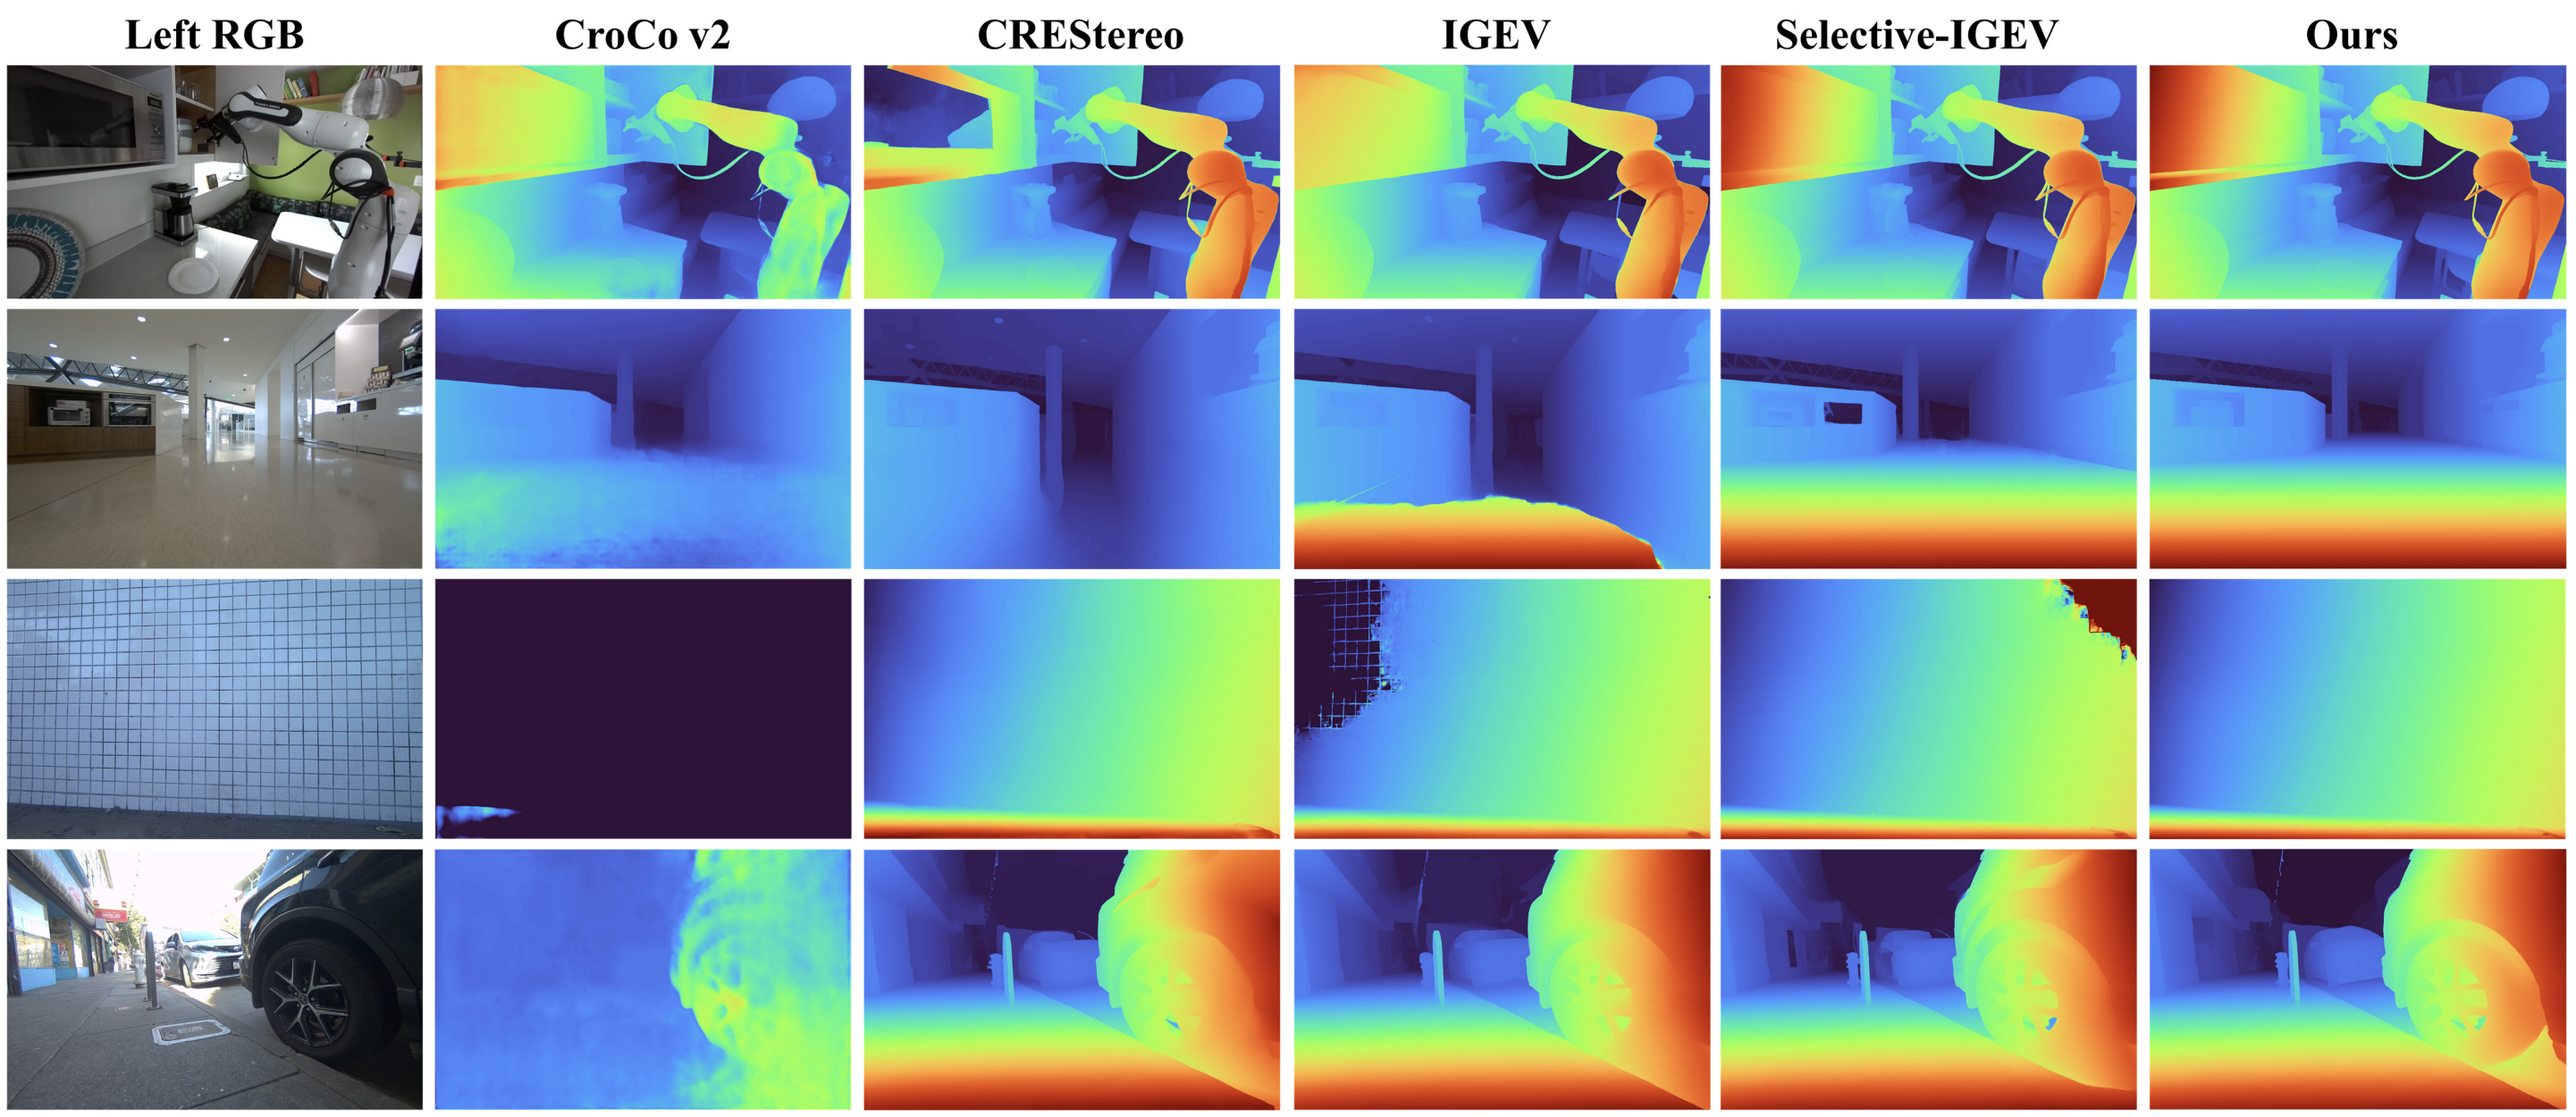
\includegraphics[width=0.95\linewidth]{../src/imports/Figure5.png}
      \end{center}
      \vspace{0.3cm}
      Sharp, detailed disparity maps with accurate boundaries. Better handling
      of reflections, thin structures, and textureless regions.
    \end{block}

  \end{column}
  \hspace{1cm}
\end{columns}

\vspace{0.8cm}

% =============================================================================
% FOOTER
% =============================================================================
\begin{beamercolorbox}[wd=\paperwidth, leftskip=2.5cm, rightskip=2.5cm, vmode]{block title}
  \vspace{0.8cm}
  \begin{columns}[t, totalwidth=\dimexpr\paperwidth-5cm\relax]
    \begin{column}{0.48\linewidth}
      {\large\bfseries Key Takeaways}\par
      \vspace{0.3cm}
      {\small
        \checkmark\ \textbf{Foundation model paradigm} works for stereo\par
        \vspace{0.2cm}
        \checkmark\ \textbf{Large-scale synthetic data} + monocular priors enable zero-shot transfer\par
        \vspace{0.2cm}
        \checkmark\ \textbf{Hybrid reasoning} crucial for robust cost volumes
      }
    \end{column}
    \begin{column}{0.48\linewidth}
      {\large\bfseries Limitations}\par
      \vspace{0.3cm}
      {\small
        \textbullet\ \textbf{Efficiency:} Transformer modules need optimization for real-time\par
        \vspace{0.2cm}
        \textbullet\ \textbf{Transparent objects:} Limited glass/water diversity in training
      }
    \end{column}
  \end{columns}
  \vspace{0.8cm}
\end{beamercolorbox}

\end{frame}
\end{document}
